\documentclass[9pt]{IEEEtran}

\usepackage[english]{babel}
\usepackage{graphicx}
\usepackage{epstopdf}
\usepackage{fancyhdr}
\usepackage{amsmath}
\usepackage{amsthm}
\usepackage{amssymb}
\usepackage{url}
\usepackage{array}
\usepackage{textcomp}
\usepackage{listings}
\usepackage{hyperref}
\usepackage{xcolor}
\usepackage{colortbl}
\usepackage{float}
\usepackage{gensymb}
\usepackage{longtable}
\usepackage{supertabular}
\usepackage{multicol}
\usepackage{tabu}
\usepackage{verbatim}


\usepackage[utf8x]{inputenc}

\usepackage[T1]{fontenc}
\usepackage{lmodern}
\input{glyphtounicode}
\pdfgentounicode=1



\DeclareGraphicsExtensions{.pdf,.png,.jpg,.eps}

% correct bad hyphenation here
\hyphenation{op-tical net-works semi-conduc-tor trig-gs}

% ============================================================================================

\title{\vspace{0ex}
Indexer}

\author{Timotej Kovač\vspace{-4.0ex}}

% ============================================================================================

\begin{document}

\maketitle

\section{Introduction}

In this paper we describe the results gathered while testing two approaches in finding relevant documents to a search query.
The two approaches used were the invert index and a manual checking one.
We describe the implementation of both of them, pre-processing steps that were taken before and the results that we got. 

\section{Indexer implementation}

\subsection{Data processing with indexing}

All of the data pre-processing was done in file \verb+processing.py+.
There html content is read directly from file and a DOM tree is constructed with the help of 'lxml.html' library.
This is then cleaned of all scripts and nav and footer sub trees.
After that only the body is forwarded to the next step of the extraction process.
The result is then tokenized with the help of 'nltk' library, special characters are removed with the help of regular expressions library 're' and the resulting words are checked with the stop words black list.
After this process what remains are only the words that have some meaning and are deemed useful for indexing.
This was done for all of the websites that were available to us.

After that the unique words were gathered and tuples were created in order to insert them into the database.
First two tables \verb+IndexWord+ and \verb+Posting+ were created.
After that all of the data was inserted with two insert statements.
This was necessary as individual insert statements which were first executed during the word tokenization proved to be inefficient.

\subsection{Data retrieval with inverted index}

For the data retrieval part with the help of mySQL database we started by retrieving the user input query words.
First we checked if the database was present and if necessary we ran the data processing step with indexing (as described in the previous section).
After that multiple select statements were executed to gather the frequency, document and indices of particular words appearing in the previously retrieved html pages.
After that all of the data for individual query words were merged and sorted from the most frequent ones to least.
Snippets were extracted to be attached to the end result.
At the end the retrieved data was formatted and sent to the standard output.

\subsection{Data retrieval without inverted index}

For this part we used some of the same approaches as when we used the inverted index database.
The main difference here was that we didn't use the database so we didn't have to create it and fill it with data.
Nevertheless we still had to gain information about the appearance of words in html pages.
So we started with this extraction and then manually checked each result if any of the query words appeared in it.
If this was the case we saved the frequency, document and indices and proceeded with the search.
After searching all of the documents we proceeded with merging the results, adding snippets, sorting them, formatting the output and sending everything to the standard output.

\section{Database description}

From the html pages we have extracted a total of 48.081 unique words that were then saved to IndexWord table.
Word with the highest frequency on a given site was 'proizvodnja' with a frequency of 2266 on site evem.gov.si.
Word with the highest frequency over all the sites was 'slovenije' with a frequency of 9105.

\section{Results}

From the results it is apparent that the approach using the inverted index data is far superior to the one that manually checks all of the documents.
Time needed for each approach can be seen in table ~\ref{tab1}.

\begin{table}[ht]
\begin{tabu} to 1.0\columnwidth {|X[l]| X[l] | X[l] |}
\hline
query/method            & inverted index & manual checking \\ \hline
predelovalne dejavnosti &      19ms   (20ms)       &           92085ms      \\ \hline
trgovina                &      4ms     (5ms)     &         92414ms        \\ \hline
social services         &       69ms    (5ms)     &         92335ms        \\ \hline
robot                       &        124ms (5ms)        &          92516ms       \\ \hline
davčna olajšava           140ms   (5ms)         &        93280ms        &                 \\ \hline
podatki                       &         24ms (20ms)      &        93650ms         \\ \hline
\end{tabu}
\label{tab1}
\caption{Comparison of time needed to gain a query result using the inverted index and manual checking methods. In brackets is the time needed only for the SQL query without any post-processing.}
\end{table}

From the table it can be seen that manual checking roughly takes the same amount of time regardless of the input.
That is because it must check all of the document as it does not know which contain any of the query words.
The inverted index method takes a much smaller amount of time. 
This time does vary a lot but always performs in under 200ms while the manual approach takes a minute and a half.

The actual results gathered using the inverted index for the above mentioned queries can be seen in the following subsections.
The outputs have been cut to only keep the top 10 results and maximum of 5 snippets.

\onecolumn
\subsection{predelovalne dejavnosti}

Result of query 'predelovalne dejavnosti'.
\begin{figure}[ht]
    \centering
    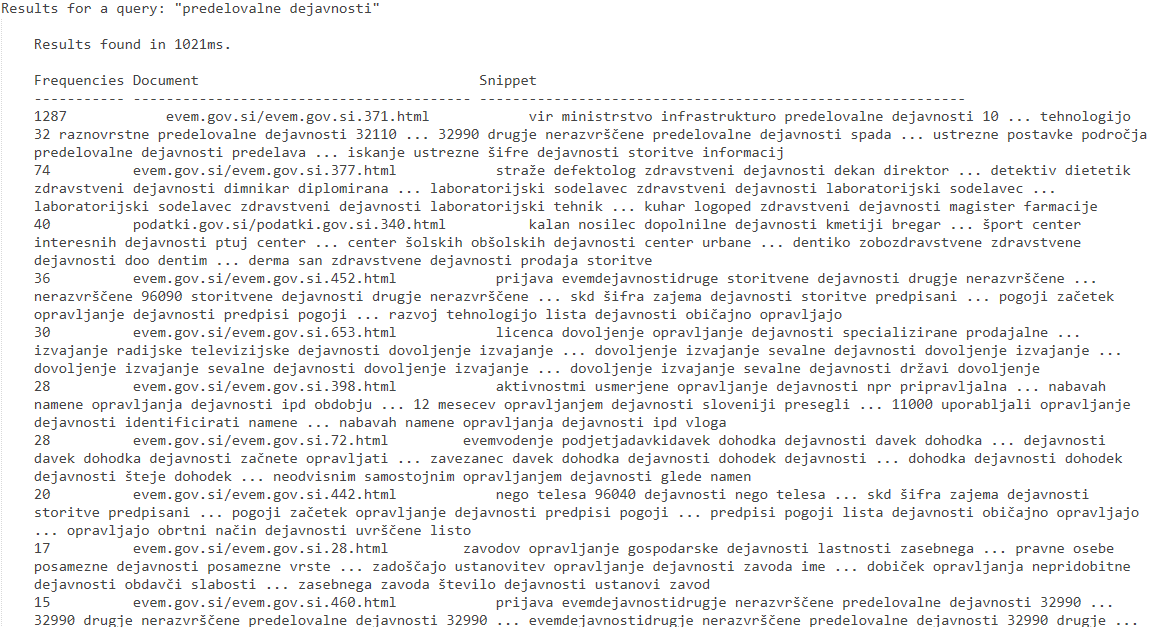
\includegraphics[width=1\columnwidth]{predelovalne_dejavnosti.png}
    \label{fig1}
\end{figure}
\clearpage

\subsection{trgovina}

Result of query 'trgovina'.
\begin{figure}[ht]
    \centering
    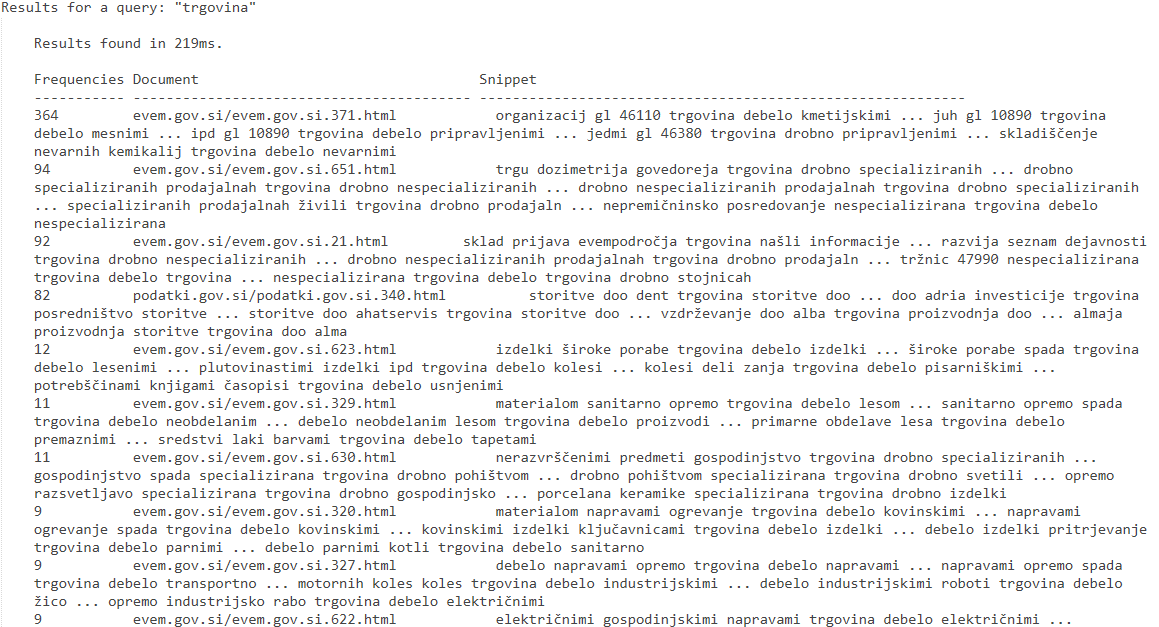
\includegraphics[width=1\columnwidth]{trgovina.png}

    \label{fig2}
\end{figure}


\subsection{social services}

Result of query 'social services'.
\begin{figure}[ht]
    \centering
    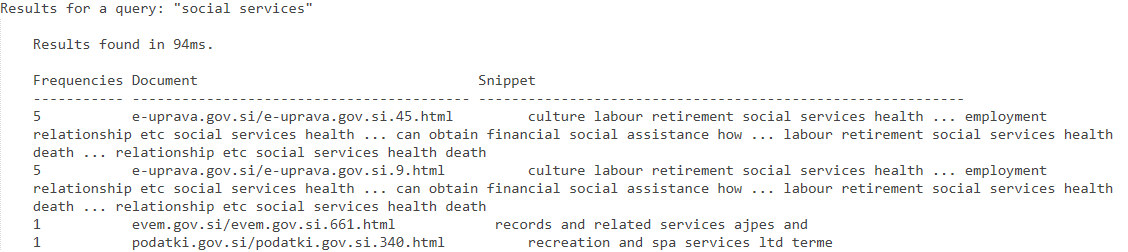
\includegraphics[width=1\columnwidth]{social_services.png}

    \label{fig3}
\end{figure}

\clearpage

\subsection{robot}
Result of query 'robot'.
\begin{figure}[ht]
    \centering
    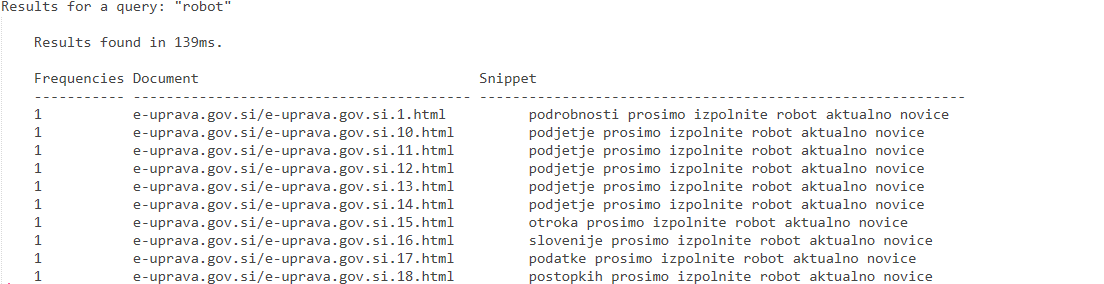
\includegraphics[width=1\columnwidth]{robot.png}

    \label{fig4}
\end{figure}


\subsection{davčna olajšava}
Result of query 'davčna olajšava'.
\begin{figure}[ht]
    \centering
    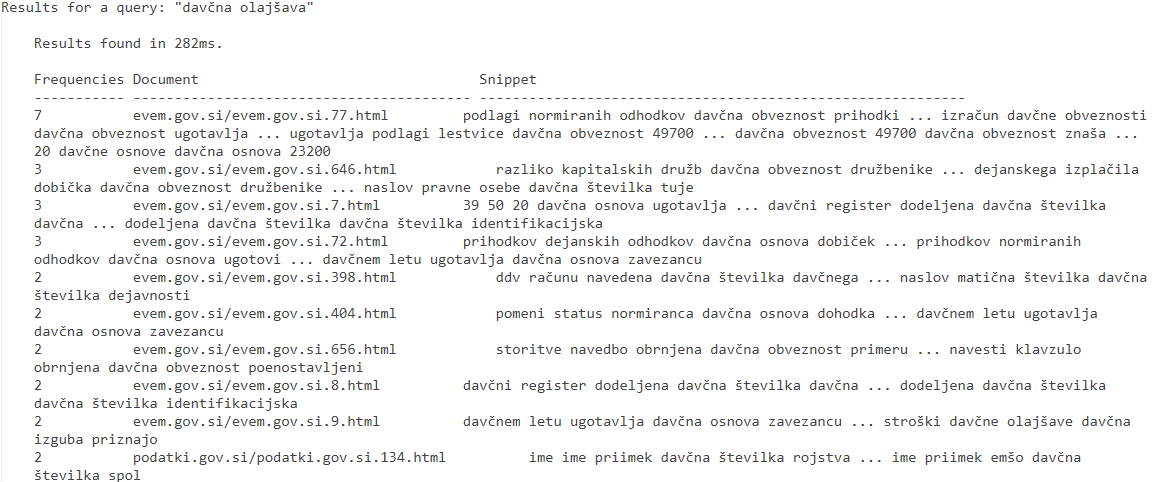
\includegraphics[width=1\columnwidth]{davcna_olajsava.png}

    \label{fig5}
\end{figure}
\clearpage

\subsection{podatki}

Result of query 'podatki'.
\begin{figure}[ht]
    \centering
    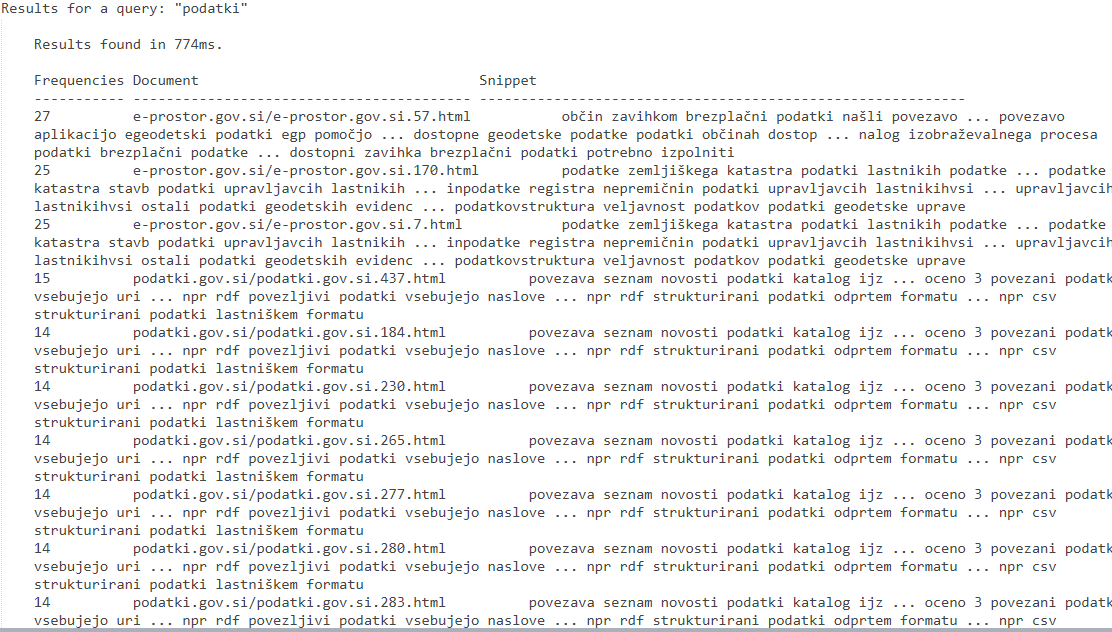
\includegraphics[width=1\columnwidth]{podatki.png}

    \label{fig6}
\end{figure}
\clearpage

\twocolumn
\section{Conclusion}

We were successful in implementing the invert index approach as well as the manual checking one.
The results we got are in favor to the invert index one as it is clearly much faster and far less demanding as the manual checking one.
With further improvements to database structure and better pre-processing steps we could improve the time needed for a search result execution.

\bibliographystyle{IEEEtran}
\bibliography{main}

\end{document}
